\documentclass[11pt]{article}
\usepackage[margin=1in, headheight=14pt]{geometry}
\usepackage{amsmath, amssymb}
\usepackage{hyperref}
\usepackage{enumitem}
\usepackage{algorithm}
\usepackage{algpseudocode}
\usepackage{fancyhdr}
\usepackage{tcolorbox}
\usepackage{microtype}
\usepackage{tikz}
\usepackage{pgfplots}
\pgfplotsset{compat=1.18}
\usetikzlibrary{arrows.meta, positioning, calc, shapes.geometric}

\input{notation.tex}
\input{zk-notation.tex}
\input{environments.tex}
\input{lecture-macros.tex}

\pagestyle{fancy}
\fancyhf{}
\lhead{EECS 498/CSE 598: Zero-Knowledge Proofs}
\rhead{Winter 2026}
\lfoot{Lecture 19: Non-Native Arithmetic, Composite Proofs, and Parsing}
\rfoot{\thepage}
\renewcommand{\headrulewidth}{0.4pt}
\renewcommand{\footrulewidth}{0.4pt}

% Lecture-specific macros
\tcbuselibrary{skins, breakable}

\newtcolorbox{highlight}[1][]{
  colback=blue!5!white,
  colframe=blue!60!black,
  fonttitle=\bfseries,
  #1
}

\newcommand{\DFA}{\ensuremath{\mathsf{DFA}}}
\newcommand{\NFA}{\ensuremath{\mathsf{NFA}}}
\newcommand{\XJsnark}{\ensuremath{\mathsf{xJsnark}}}

\begin{document}

%-----------------------------------------------------------------------
% Title Block
%-----------------------------------------------------------------------
\begin{center}
  {\LARGE \textbf{EECS 498 / CSE 598: Zero-Knowledge Proofs}}\\[6pt]
  {\large Winter 2026}\\[4pt]
  {\large \textbf{Lecture 19: Non-Native Arithmetic, Composite Proofs, and Parsing}}\\[4pt]
  {\large Instructor: Paul Grubbs \quad
    \href{mailto:paulgrub@umich.edu}{\texttt{paulgrub@umich.edu}} \quad
    Beyster 4709}
\end{center}

\vspace{0.5em}
\hrule
\vspace{1em}

%-----------------------------------------------------------------------
% Agenda
%-----------------------------------------------------------------------
\section*{Agenda}
\begin{itemize}
  \item Motivation and recurring frontend bottlenecks
  \item Non-native arithmetic with small and large target moduli
  \item Composite proofs for mixed-arithmetic statements
  \item Parsing and string operations
  \item Proving finite-automaton executions
  \item General representation issues and applications
\end{itemize}

\hrule
\vspace{1em}

%-----------------------------------------------------------------------
\section{Motivation}
%-----------------------------------------------------------------------

Several natural zero-knowledge statements fall outside the most convenient
native arithmetic model of an \algo{R1CS} over a field $\F_p$:
\begin{itemize}
  \item knowledge of an \algo{RSA} signature $\sigma$ on a message $m$;
  \item compliance of an \algo{HTTP} header with a network policy;
  \item satisfaction of a regular expression by a private document;
  \item validity of a signed \algo{JSON} blob containing an age claim;
  \item knowledge of $x \in \F$ such that $s = H(xG)$ for a public hash output $s$.
\end{itemize}

The examples separate into three structural challenges.  Some computations use
integers or rings much larger than the native field of the proof system, some
operate on structured strings rather than field elements, and some mix several
algebraic domains in one statement.

\begin{highlight}[title={Three Structural Strategies}]
Statements of this kind are handled with three recurring design patterns:
\begin{enumerate}
  \item encode non-native arithmetic inside \algo{R1CS};
  \item split a mixed computation across several proof systems and combine the
        resulting subproofs with a consistency check;
  \item represent parsing and string operations with circuit-friendly state
        machines, tables, or lookup constraints.
\end{enumerate}
\end{highlight}

The underlying theme is that the native representation of the proof system is
rarely the native representation of the application.  Efficiency depends on how
the application is recast into arithmetic constraints.

%-----------------------------------------------------------------------
\section{Non-Native Arithmetic}
%-----------------------------------------------------------------------

\begin{definition}[Non-native arithmetic]
Non-native arithmetic is arithmetic performed over a ring or field different
from the native field $\F_p$ of the proof system.
\end{definition}

The most common cases split according to the size of the target modulus $m$
relative to $p$:
\begin{itemize}
  \item the \emph{small-modulus case}, where $m \ll p$ and integer operations
        fit comfortably inside one native field element;
  \item the \emph{large-modulus case}, where $m \gg p$ and values must be
        represented across several limbs;
  \item extension-field settings such as $\mathrm{GF}(2^{128})$, where the
        algebraic structure differs from prime-field arithmetic even when the
        bit lengths are comparable.
\end{itemize}

\subsection{The Small-Modulus Case}

When $m$ is much smaller than $p$, native field arithmetic can be used as
ordinary integer arithmetic, provided that the circuit enforces suitable range
bounds.  For example, the relation
\[
  c = a + b \bmod 2^{32}
\]
can be enforced by introducing a carry bit $k$ and checking
\[
  a + b = c + k \cdot 2^{32},
  \qquad
  k \in \{0,1\}.
\]

\begin{proposition}
Let $a,b,c \in [0,2^{32}-1]$.  Then
\[
  c = a + b \bmod 2^{32}
\]
holds if and only if there exists $k \in \{0,1\}$ such that
\[
  a + b = c + k \cdot 2^{32}.
\]
\end{proposition}

\begin{proof}
If $c$ is the reduction of $a+b$ modulo $2^{32}$, then the quotient in the
division of $a+b$ by $2^{32}$ is either $0$ or $1$ because
\[
  0 \leq a+b \leq 2^{33}-2.
\]
Therefore $a+b = c + k 2^{32}$ for some $k \in \{0,1\}$.  The converse is
immediate after reducing both sides modulo $2^{32}$.
\end{proof}

In a circuit, the resulting local check is therefore
\[
  a+b=c+k2^{32},
  \qquad
  k(k-1)=0,
  \qquad
  0 \leq a,b,c < 2^{32}.
\]
This cost profile is the main reason lookup arguments are useful in this
setting.  The slide deck emphasizes that range checking often accounts for
nearly all of the cost of small-modulus arithmetic gadgets, so faster lookup-
based range proofs produce most of the savings.

\subsection{The Large-Modulus Case}

When $m$ is much larger than $p$, a single field element can no longer hold one
target value.  A standard representation writes
\[
  x = x_0 + x_1 B + \cdots + x_{d-1} B^{d-1},
\]
where $B$ is a limb base and each $x_i$ is constrained to lie in a suitable
interval.

Addition and subtraction modulo $m$ then become limb-wise operations with
carry propagation.  The main difficulty is multiplication.  The slide deck
describes the \XJsnark{} viewpoint: interpret the limb vectors of $x$, $y$, and
$z$ as coefficient vectors of univariate polynomials
\[
  X(T) = \sum_{i=0}^{d-1} x_i T^i,
  \qquad
  Y(T) = \sum_{i=0}^{d-1} y_i T^i,
  \qquad
  Z(T) = \sum_{i=0}^{2d-2} z_i T^i.
\]
The coefficient identity corresponding to the integer product of the limb
vectors can be checked by evaluating these polynomials at sufficiently many
points.

\begin{proposition}
Suppose $X(T)$ and $Y(T)$ have degree at most $d-1$, and $Z(T)$ has degree at
most $2d-2$.  Then the polynomial identity
\[
  X(T)Y(T)=Z(T)
\]
is determined by its values on any set of at least $2d-1$ distinct points.
\end{proposition}

\begin{proof}
The polynomial $X(T)Y(T)-Z(T)$ has degree at most $2d-2$.  A nonzero polynomial
of degree at most $2d-2$ cannot vanish on $2d-1$ distinct points.  Therefore
vanishing on any larger evaluation set, including the slide choice
\[
  c \in \{0,\ldots,2d-1\},
\]
forces the identity to hold identically.
\end{proof}

For modular multiplication,
\[
  x \cdot y = z \bmod m,
\]
the witness supplies a quotient $q$ and the circuit checks
\[
  x \cdot y = q m + z
\]
in the large-integer representation, together with the relevant range bounds on
the limbs of $q$ and $z$.  The same polynomial-evaluation idea reduces the
constraint cost of the multiplication itself, while range conditions and carry
constraints maintain correctness of the limb encoding.

The unresolved design parameter is the limb size.  Large limbs reduce the
number of limbs but tighten the native-field headroom available for carry
management.  Small limbs simplify carry constraints but enlarge the witness and
the multiplication machinery.  Efficient non-native arithmetic is largely the
problem of balancing those two pressures.

%-----------------------------------------------------------------------
\section{Composite Proofs}
%-----------------------------------------------------------------------

Some statements mix several kinds of computation so unevenly that no single
proof system is a good fit for all of them.  A typical example combines a
hash-based relation over elliptic-curve data with ordinary arithmetic or with a
string-processing task.

The slide deck presents a generic decomposition pattern.  Let the target
relation have the form
\[
  R(x)=1
  \iff
  \exists\, w_s,w_1,w_2
  \text{ such that }
  R_1(x,w_s,w_1)=1
  \text{ and }
  R_2(x,w_s,w_2)=1,
\]
where $w_s$ is the witness component shared by the two subrelations.  The
prover then generates proofs
\[
  \pi_1 \leftarrow \algo{P}_1(x,w_s,w_1),
  \qquad
  \pi_2 \leftarrow \algo{P}_2(x,w_s,w_2),
\]
and adds a cheap consistency check showing that the two subproofs refer to the
same shared witness component $w_s$.

\begin{center}
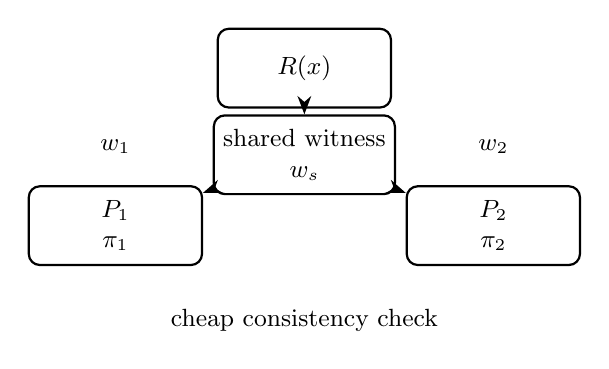
\begin{tikzpicture}[
  box/.style={draw, thick, rounded corners, minimum width=2.2cm, minimum height=1cm, align=center},
  arr/.style={-Stealth, thick},
  every node/.style={font=\small}
]
  \node[box] (R) at (0,2.0) {$R(x)$};
  \node[box] (P1) at (-2.4,0) {$\algo{P}_1$\\$\pi_1$};
  \node[box] (P2) at ( 2.4,0) {$\algo{P}_2$\\$\pi_2$};
  \node[box] (Ws) at (0,0.9) {shared witness\\$w_s$};
  \node at (-2.4,1.0) {$w_1$};
  \node at ( 2.4,1.0) {$w_2$};
  \node at (0,-1.2) {cheap consistency check};
  \draw[arr] (R) -- (Ws);
  \draw[arr] (Ws) -- (P1);
  \draw[arr] (Ws) -- (P2);
\end{tikzpicture}

\smallskip
\emph{Composite-proof structure with a shared witness component.}
\end{center}

\begin{proposition}
If both subproof systems are sound for $R_1$ and $R_2$, and the consistency
check soundly enforces equality of the shared witness component, then the
combined proof establishes $R(x)=1$.
\end{proposition}

\begin{proof}[Proof sketch]
Soundness of the two subproof systems yields witnesses
\[
  (w_s^{(1)},w_1)
  \qquad\text{and}\qquad
  (w_s^{(2)},w_2)
\]
for the two subrelations.  The consistency check forces
$w_s^{(1)}=w_s^{(2)}$, so there is one shared witness $w_s$ satisfying both
subrelations simultaneously.  Therefore the combined witness
\[
  (w_s,w_1,w_2)
\]
satisfies $R$.
\end{proof}

Composite proofs are especially attractive when the mismatch between proof
systems is structural rather than accidental.  One subrelation may be best
handled in an \algo{R1CS}, while another is more naturally expressed over a
different algebraic domain or through a specialized argument for tables,
automata, or commitments.

%-----------------------------------------------------------------------
\section{Parsing and String Operations}
%-----------------------------------------------------------------------

Structured-data proofs introduce a second source of difficulty: the witness is
often not naturally a tuple of field elements, but a document or byte string.
The slide ordering is useful:
\begin{enumerate}
  \item substring containment;
  \item regular-expression match or non-match;
  \item extraction of one field from a structured object;
  \item full parsing with respect to a grammar.
\end{enumerate}

These tasks increase in difficulty because they demand more context integrity.
A proof of substring containment only certifies that a pattern occurs
somewhere.  A proof about a field inside a structured object must also certify
that the extracted bytes occur in the right syntactic position.  Full parsing
requires global agreement with the grammar rather than one local check.

The slide annotations add two common refinements:
\begin{itemize}
  \item a \emph{partial parse}, where only the part of the grammar needed to
        justify one claim is verified;
  \item \emph{representation conversion}, such as hexadecimal or Base64
        decoding, which is naturally implemented with lookup tables.
\end{itemize}

For committed documents, the relevant circuit typically exposes the characters
or bytes only to the prover while keeping the document itself hidden.  The
proof then certifies a predicate of the committed data rather than revealing
the data itself.

%-----------------------------------------------------------------------
\section{Proving DFA Executions}
%-----------------------------------------------------------------------

Regular-expression checks are commonly reduced to automata.  The document is a
sequence
\[
  c_1,\ldots,c_n
\]
over an alphabet $\Sigma$, and the automaton state evolves according to a
transition function
\[
  T : Q \times \Sigma \to Q.
\]

For a deterministic automaton, the witness contains states
\[
  \algo{st}_0,\algo{st}_1,\ldots,\algo{st}_n
\]
such that
\[
  \algo{st}_{i+1}=T(\algo{st}_i,c_i)
  \qquad\text{for all } i=0,\ldots,n-1.
\]
Acceptance is enforced by checking that the final state lies in the accepting
set.

\begin{proposition}
Let $\calA=(Q,\Sigma,T,q_0,F)$ be a deterministic finite automaton.  If a
circuit verifies
\[
  \algo{st}_0=q_0,
  \qquad
  \algo{st}_{i+1}=T(\algo{st}_i,c_i)
  \text{ for all } i,
  \qquad
  \algo{st}_n \in F,
\]
then the input string $c_1\cdots c_n$ is accepted by $\calA$.
\end{proposition}

\begin{proof}
The checked recurrence is exactly the transition semantics of a \DFA.  The
state sequence therefore coincides with the unique execution of $\calA$ on the
input string.  The final-state check implies acceptance.
\end{proof}

The main circuit cost lies in encoding the transition function.  The slides
describe the direct implementation as a large disjunction over state-symbol
pairs:
\[
  \text{if } \algo{st}=i \text{ and } c=s,\ \text{ then } \algo{st}'=j.
\]
This implementation is conceptually straightforward but can be expensive for
large state spaces or alphabets.  A table-based or lookup-based encoding is
often preferable when the transition relation is large and regular.

Non-deterministic automata can be handled as well, but the witness must then
include enough information to justify one accepting path or an equivalent
deterministic simulation.  The underlying proof obligation remains the same:
the transition sequence must respect the automaton semantics while preserving
privacy of the committed document.

%-----------------------------------------------------------------------
\section{Other Issues and Applications}
%-----------------------------------------------------------------------

The lecture examples all illustrate the same design pressure.  Proof systems
operate natively on one arithmetic representation, while applications rarely do.
\algo{RSA} signatures require large-modulus arithmetic.  \algo{HTTP} policies and
regular expressions require string processing.  Signed \algo{JSON} objects mix
cryptography, parsing, and context integrity.  Elliptic-curve hash relations can
mix group arithmetic with field arithmetic inside one statement.

\begin{remark}
Representation is not a cosmetic choice.  It determines which constraints are
local, which subcomputations require special gadgets, and whether one proof
system is sufficient or a composite proof is needed.
\end{remark}

\end{document}
